\documentclass{article}

\usepackage[spanish]{babel}
\usepackage[numbers,sort&compress]{natbib}
\usepackage{graphicx}
\usepackage{subfigure}
\usepackage{url}
\usepackage{amsmath}
\usepackage{hyperref}
\usepackage[top=15mm, bottom=40mm, left=15mm, right=15mm]{geometry}
\setlength{\parskip}{2mm}
\setlength{\parindent}{0pt}



\author{Dulce Esperanza Carrasco Castillo 1445183}
\title{Práctica 2: autómata celular}
\date{\today}

\begin{document}

\maketitle


\section{Descripción}
Usando R se hace una malla de 30 por 30 celdas, se varía la probabilidad inicial de 0 a 1 en cada corrida \cite{elisaweb}, después se ajustan los valores para indicar que una celda está viva (1) ó muerta (0) junto con los pasos requeridos, en este caso de 0.1; con lo anterior establecido se va variando el número de iteraciones, de manera que cada celda vive o muere dependiendo del tipo de celdas que tenga como vecinas. El número de iteraciones se determina cuando las celúlas (celdas) mueren, esto se puede observar en R por el número de veces que aparece el escrito "Ya no queda nadie vivo".

\section{Resultados}

En la figura \ref{cajabigote} se muestran los resultados donde el eje y son las iteraciones y el eje x la probabilidad inicial de 0.0 a 1.0 donde 1=0.0, 2=0.1, 3=0.2, etc.

\begin{figure}
\centering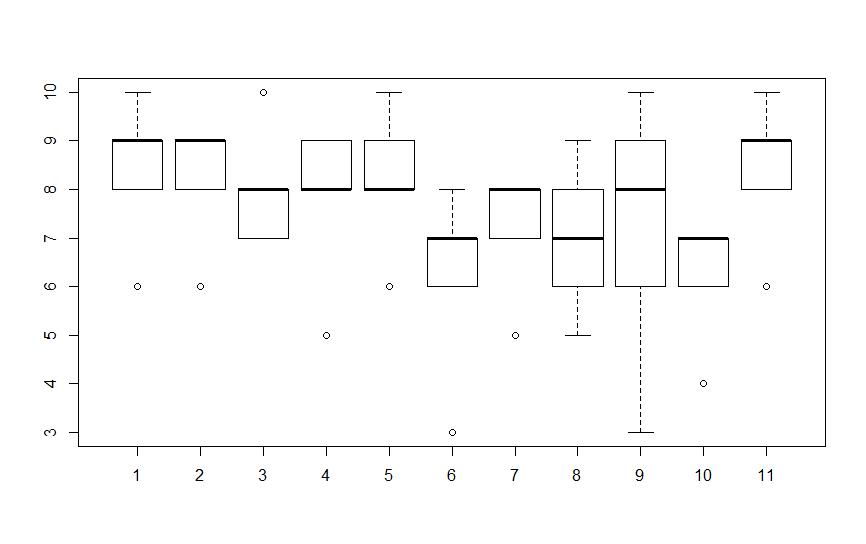
\includegraphics[width=160mm]{p2cajabigote.png}
\caption{Iteraciones}
\label{cajabigote}
\end{figure}











\bibliographystyle{plainnat}
\bibliography{p2}

\end{document}